
%(BEGIN_QUESTION)
% Copyright 2007, Tony R. Kuphaldt, released under the Creative Commons Attribution License (v 1.0)
% This means you may do almost anything with this work of mine, so long as you give me proper credit

Data in an Ethernet network is transmitted in a series of bits known as a {\it frame}.  A basic organizational illustration for an Ethernet frame is as follows (according to the IEEE 802.3 standard):

$$\includegraphics[width=15.5cm]{i02204x01.eps}$$

Explain the purpose of each frame section:

\begin{itemize}
\item{} Preamble:
\vskip 5pt
\item{} SFD:
\vskip 5pt
\item{} Destination address:
\vskip 5pt
\item{} Source address:
\vskip 5pt
\item{} Type (or Length): 
\vskip 5pt
\item{} Data:
\vskip 5pt
\item{} Frame check sequence:
\end{itemize}

\vskip 20pt \vbox{\hrule \hbox{\strut \vrule{} {\bf Suggestions for Socratic discussion} \vrule} \hrule}

\begin{itemize}
\item{} The {\it preamble} section of an Ethernet frame is extremely important for practical reasons, although at first blush it appears to be useless (an alternating sequence of 1's and 0's?).  Explain why the preamble is a necessary component of the Ethernet frame.
\item{} Ethernet data frames do not use a ``parity'' bit as is the case with data frames of RS-232 and other (simpler) serial network standards.  Why is a parity bit unnecessary with Ethernet?  Explain why a parity bit would be far less useful (if it was used) in Ethernet than it is in an RS-232 data frame.
\end{itemize}

\underbar{file i02204}
%(END_QUESTION)





%(BEGIN_ANSWER)

\noindent
{\bf Partial answer:}

\vskip 10pt

\begin{itemize}
\item{} Preamble:
\vskip 5pt
\item{} SFD: {\it Start-of-Frame Delimiter, to signal the end of the preamble bitstream.}
\vskip 5pt
\item{} Destination address: {\it the MAC address of the intended recipient.}
\vskip 5pt
\item{} Source address: {\it the MAC address of the transmitting station.}
\vskip 5pt
\item{} Type (or Length): {\it contains a code to specify the purpose of the data bits, or a code specifying the number of data bytes contained in the Data field.  This can be either, depending on the value of the code.  If 1500 or less, it represents the Data field length; if 1536 or more, it represents data type (assumed Data field length of 46 bytes).}
\vskip 5pt
\item{} Data:
\vskip 5pt
\item{} Frame check sequence:
\end{itemize}

%(END_ANSWER)





%(BEGIN_NOTES)

\begin{itemize}
\item{} Preamble: {\it A set of alternating 1's and 0's used to synchronize the transmitting and receiving devices, also serves as a buffer against data loss in case the receiving station misses a few first bits.  Obsolete in Fast Ethernet and Gigabit Ethernet, but still maintained for backward compatibility.}
\vskip 5pt
\item{} SFD: {\it Start-of-Frame Delimiter, to signal the end of the preamble bitstream.}  (Consists of this stream: {\tt 10101011}, which is a hexadecimal {\tt AB}.
\vskip 5pt
\item{} Destination address: {\it the MAC address of the intended recipient.}
\vskip 5pt
\item{} Source address: {\it the MAC address of the transmitting station.}
\vskip 5pt
\item{} Type (or Length): {\it contains a code to specify the purpose of the data bits, or a code specifying the number of data bytes contained in the Data field.  This can be either, depending on the value of the code.  If 1500 or less, it represents the Data field length; if 1536 or more, it represents data type (assumed Data field length of 46 bytes).}
\vskip 5pt
\item{} Data: {\it the data being carried by the packet.  Duh.}
\vskip 5pt
\item{} Frame check sequence: {\it also known as CRC (Cyclic Redundancy Check).  This is a code used for error detection in the data stream.}
\end{itemize}

%INDEX% Networking, Ethernet: frame

%(END_NOTES)


